\subsection{Tracking}
\label{tracking}
Die Bewegung eines starren Körpers wird mit drei Koordinaten für die Position und drei Winkeln für die Orientierung angegeben\cite*[Dörner (2019) S.119f.,][]{doerner}. Diese sechs Werte werden als \textit{Freiheitsgrade (engl. \acrfull{dof})} bezeichnet. Der Begriff Tracking beschreibt die kontinuierliche Verfolgung von Positions- und Orientierungsdaten.

Im AR Kontext wird die Position und Orientierung des Smartphones kontinuierlich berechnet. Gleichzeitig wird die Umgebung erfasst und sogenannte Schlüsselpunkte festgelegt. Anhand der Schlüsselpunkte können z.B. Flächen erkannt werden, auf denen die virtuellen Objekte platziert werden. Billinghurst\cite[][]{billinghurst2015} nennt zwei Phasen beim Tracking:

\begin{itemize}
    \item eine Registrierungsphase, bei der die Position und Orientierung des Smartphones beim Start der Anwendung im Bezug auf einem Ankerpunkt in der realen Welt bestimmt wird,
    \item eine Trackingphase, bei der die Position und Orientierung des Smartphones anhand der vorherigen Position und Orientierung aktualisiert wird.
\end{itemize}

Das Ziel beim Tracking ist es, die sechs Freiheitsgrade für die Translation und Rotation der Objekte kontinuierlich zu bestimmen bzw. zu schätzen. Die Aufnahme der Daten erfolgt durch Sensoren z.B. durch die \textit{\acrfull{imu}} in Smartphones und Tablets. Die IMU wird in Kapitel \ref*{tracking-imu} behandelt.

Es werden zwischen zwei Trackingverfahren unterschieden. Beim \textit{Outside-In-Tracking} befindet sich die Sensorik zur Datenaufnahme in der Umgebung innerhalb eines bestimmten Raumes, sodass das Objekt von außen getrackt wird. Dies wird bei VR-Brillen eingesetzt. Der Nachteil dieser Technik ist, dass die Sensoik an einem Ort gebunden ist und bei einem Ortswechsel neu platziert werden muss. Beim \textit{Inside-Out-Tracking} befinden sich Sensoren im Objekt, das getrackt werden soll. Die Position und Lage des Objekts wird im Verhältnis zur Umgebung gesetzt. Bei der AR Anwendung in dieser Arbeit handelt es sich somit um ein Inside-Out-Tracking. Vorteil dieser Methode ist, dass der Nutzer nicht an einem Ort gebunden ist. Probleme treten in der Genauigkeit beim Tracking auf. Das Tracking System im Smartphone muss sich rein auf die Sensoren in der IMU und dem Kamerabild verlassen, während beim Outside-InTracking mehr Sensoren zur Verfügung stehen.

In der Unity Manual zu AR Foundation wird der Begriff Tracking mit der Bestimmung der relativen Position und Orientierung in der physichen Welt definiert. Zusätzlich wird darauf hingewiesen, dass falls die Umgebung zu dunkel ist, das Gerät Probleme beim Tracking bekommt und die Genauigkeit der Positionsbestimmung sich verringert \cite{UnityARFoundation}. Damit ist davon auszugehen, dass in AR Foundation Kamera-basiertes Tracking (siehe Kapitel \ref*{tracking-kamerabasiertes-tracking}) verwendet wird. Kamera-basiertes Tracking wird in Kapitel \ref*{tracking-kamerabasiertes-tracking} näher behandelt.

\subsubsection{Koordinatensysteme}
\label{tracking-koordinatensysteme}
Um eine Bestimmung bzw. Schätzung der Translationen und Rotationen durchzuführen, werden zwei Koordinatensysteme herangezogen. Ein Kamerakoordinatensystem und ein Objektkoordinatensystem. Weiterhin gibt es die Möglichkeit, dass für alle Objekte im Raum ein Koordinatensystem (Weltkoordinatensystem) verwendet wird. Voraussetzung für das Tracking ist, dass die Transformationen zwischen den Objekten bekannt sind. Dann kann die Transformation zwischen dem Objekt und dem Weltkoordinatensystem geschätzt werden.\cite*[Dörner (2019) S.124f.,][]{doerner}.

In Unity und AR Foundation hat das Smartphone ein eigenes Koordinatensystem. Wird eine AR-Session gestartet, so wird ein Koordinatensystem für diese spezifische Session initialisiert. Die Koordinaten (0,0,0) stehen für die Position des Gerätes, bei dem die Session gestartet ist \cite{UnityARFoundation}. Die z-Achse zeigt dabei in die Richtung, in die die Kamera des Smartphones gerichtet ist. Dieser Umstand ist für die Roatation der Gebäude in der GPS Platzierung relevant und wird in Kapitel \ref*{umsetzung-gps-ausrichtung-nach-norden} erläutert. Die \textit{GameObjects} in der Szene haben ein lokales Objektkoordinatensystem.

\subsubsection{Tracking mit der Inertial Measurement Unit (IMU)}
\label{tracking-imu}
Eine Inertial Measurement Unit besteht typischerweise aus Beschleungungssensoren, Drehratensensoren. Drei Beschleunigungssensoren und drei Drehratensensoren werden orthogonal zueinander eingebaut. Die Sensoren bilden ein Trägheitsnavigationssystem. Dieses misst die Bewegungsrichtung, die Beschleunigung und die Drehung in einem kartesischen Koordinatensystem und bestimmt damit die Position und Orientierung der \acrshort{imu}\footnote{https://www.5gpositioning.com/inertial-measurement-units-in-smartphones/, zuletzt aufgerufen am 27.07.2022}. Die Orientierung kann anhand der Drehratensensoren präzise bestimmt werden. Die Position wird mit den Beschleunigungswerten und der dabei vergangenen Zeit pro Aktualisierung berechnet. Die Genauigkeit dieser Berechnung ist insbesondere bei niedrigpreisigen Smartphones nicht akkurat. Es kommt zu \textit{Drifteffekten}.
Dörner beschreibt den Hintergrund des Probelms präzise: 

\glqq [..] wird beispielsweise ein Sensor aus dem Ruhezustand bewegt und anschließend wieder angehalten, so müssten sowohl die Summen der erfassten Beschleunigungswerte wie auch die der errechneten Geschwindigkeitswerte am Ende Null ergeben\grqq{}\cite*[Dörner (2019) S.127f.,][]{doerner}. 
Durch die Ungenauigkeit wird dies nicht erzielt und die errechnete Position weicht von der tatsächlichen Position ab. Zur Bestimmung der Orientierung wird die IMU oft genutzt. Da in AR Anwendungen eine hohe Präzision in der Positionsbestimmung benötigt wird, wird reines IMU-Tracking nicht genutzt. Es wird zusätzliche Kamera-basiertes Tracking benötigt, um den Drifteffekt auszugleichen\cite[Billinghurst (2015),][]{billinghurst2015}.

\subsubsection{Kamera-basiertes Tracking}
\label{tracking-kamerabasiertes-tracking}
Kamera-basiertes Tracking nutzt Bilder, um die relative Position und Orientierung der Objekte zur Kamera zu bestimmen. Die Position und Orientierung der Kamera in einem Weltkoordinatensystem wird von Hartley und Zisserman als extrinsische Kameraparameter bezeichnet \cite*[Hartley, Zisserman (2003) S.156,][]{hartleyzisserman}. Für das Kamera-basierte Tracking wird zwischen Marker-basierten und Marker-less Tracking unterschieden.

Beim Marker-basierten Tracking werden Marker (sogenannte Kanji und Hiro Marker) wie in Abbildung \ref{fig: tracking_kanji_hiro} zu sehen genutzt. Billinghurst\cite[][]{billinghurst2015} bezeichnet dies als \textit{Fiducial Tracking}. Dabei werden künstliche Marker in der Umgebung platziert. Sie dienen als Ursprung, sodass diese als als Orientierungshilfen fungieren. Populär wurde die Methode durch ARToolkit, das von Kato und Billinghurst\cite[(1999),][]{kato1999} entwickelt wurde. Das jeweilige Muster und die Größe der Marker müssen für das Tracking bekannt sein. Der Tracking Prozess ist in Abbildung \ref*{fig: tracking_ARToolkit} zu sehen. Zunächst wird das Bild im Videodatenstrom binarisiert. Die Ränder des Markers werden identifiziert. Anschließend wird die Position und die Orientierung relativ zur Kamera berechnet. Die Symbole im Marker werden mit den bekannten Symbolen aus der Datenbank verglichen und gematched. Letzlich wird  das virtuelle Objekt mit der Position und Orientierung des Markers transformiert und in das Kamerabild gerendert.

\begin{figure}[H]
    \centering
    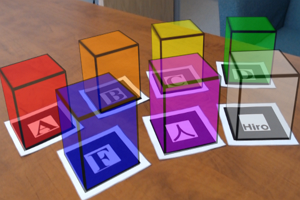
\includegraphics[width=7cm]{img/tracking/kanjo-hiro-marker.png}
    \caption[Kanji und Hiro Marker haben einfache geometrische Formen, Texte oder Buchstaben zur Erkennung in der Szene.]{Kanji und Hiro Marker haben einfache geometrische Formen, Texte oder Buchstaben zur Erkennung in der Szene\protect\footnotemark.}
    \label{fig: tracking_kanji_hiro}
\end{figure}
\footnotetext{Quelle Bild: https://stemkoski.github.io/AR-Examples/, zuletzt aufgerufen am 29.07.2022}
\begin{figure}[H]
    \centering
    \includegraphics[width=\textwidth]{img/tracking/tracking-ARToolkit.jpg}
    \caption{Der Tracking Prozess von ARToolkit\cite*[Billinghurst(2015),][]{billinghurst2015}.}
    \label{fig: tracking_ARToolkit}
\end{figure}

Die Methode ist simpel und bietet eine hohe Genauigkeit beim Tracking. Da die Marker aktiv in der Umgebung platziert werden müssen, gibt es Einschränkungen in der Flexibilität. Daher wird bei der zweiten Möglichkeit über Algorithmen der Computer Vision Merkmale in der realen Umgebung erfasst. Dies wird als \textit{marker-less AR} bezeichnet. Diese Merkmale sind Punkte oder Ecken, die aus der Umgebung herausstechen und als einzigartigen Punkt gelten. Sie sind natürliche Marker in der Umgebung. In den folgenden Kapiteln werden natürliche Merkmals-Detektoren benannt und deren Funktionsweise anhand des \acrfull{sift} Algorithmus erklärt.

\subsubsubsection{Schlüsselpunkte detektieren (Feature Detection)}
Merkmale oder auch \textit{keypoint features} oder \textit{interest points} sind Bildbereiche mit einem zentralen Punkt, die einen hohen Wiedererkennungswert besitzen. In Abbildung \ref*{fig: tracking_feature_detection_prinzip} wird deutlich, dass Flächen ohne Texturen schwer identifiziert und abgeglichen werden können. Dieses Problem ist als \textit{aperture Problem} bekannt. Erst durch starke Kontraständerungen an der Richtung der Normalen zur Kante\footnote{die durch Gradienten erkannt werden. Ein Gradient bestimmt die Richtung und Steigung der größten Änderung.}, werden Merkmale erkannt\cite[Szeliski(2022) Seite 337f., ][]{szeliski2022}. 

\begin{figure}[H]
    \centering
    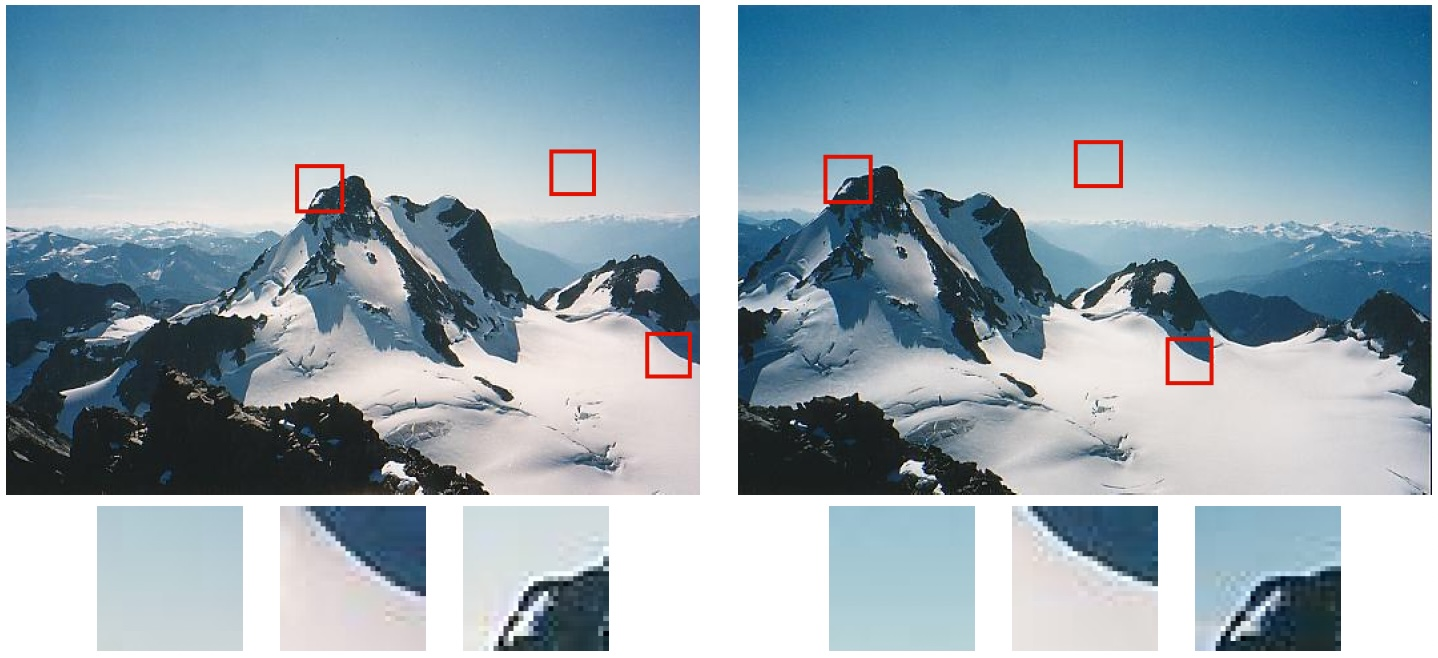
\includegraphics[width=\textwidth]{img/tracking/Feature-detection-problem.jpg}
    \caption[Die Wahrscheinlichkeit, dass eine Fläche aus dem linken Bild im rechten Bild genau identifiziert werden kann steigt, wenn starke Kontraständerungen (Gradienten) im Teilbild vorhanden sind.]{Die Wahrscheinlichkeit, dass eine Fläche aus dem linken Bild im rechten Bild genau identifiziert werden kann steigt, wenn starke Kontraständerungen (Gradienten) im Teilbild vorhanden sind\protect\footnotemark.}
    \label{fig: tracking_feature_detection_prinzip}
\end{figure}

\footnotetext{Quelle Bild: \cite*[Szeliski(2022) Seite 337,][]{szeliski2022}}

Es wird zwischen \textit{Eckendetektoren} und \textit{Blob Detektoren} unterschieden. Bekannte Kantendetektoren sind z.B.:
\begin{itemize}
    \item Harris\cite*{harris1988},
    \item \acrfull{fast} von Rosten und Drummond\cite[][]{rosten2005}.
\end{itemize}
Bekannte Blob-Detektoren sind z.B.:
\begin{itemize}
    \item \acrfull{sift} von Lowe\cite{lowe1999},
    \item \acrfull{surf} von Bay u.a.\cite{bay2008},
    \item \acrfull{orb} von Rublee u.a.\cite{rublee2011}.
\end{itemize}

Herling und Broll\cite{herling2011} nennen Herausforderungen für Detektoren, damit eine valide Position und Orientierung berechnet werden kann:
\begin{itemize}
    \item Da AR in Echtzeit abläuft, muss die Bestimmung von Schlüsselpunkten und Deskriptoren schnell berechnet werden,
    \item der Algorithmus muss robust gegenüber unterschiedlichen Lichtverhältnissen. Dies gilt insbesondere bei AR in freier Umgebung, da eine hohe Dynamik herrscht und die Lichtverhältnisse sich schnell verändern können,
    \item da der Nutzer keine Einschränkungen in der Position der Kamera besitzt, kann ein schneller Perspektivwechsel erfolgen. Der Algorithmus muss daher eine Robustheit genüber starken Bildveränderungen haben,
    \item es muss eine Skalierungsinvarianz bereitgestellt werden. Das bedeutet im \acrshort{ar} Kontext, dass das Tracking nicht auf eine bestimmte Entfernung beschränkt ist und weiter entfernte Punkte nicht verschwinden. In einem abgegrenzten Bereich ist es einfacher Schlüsselpunkte zu detektieren. Die Skaleninvarianz ist daher insbesondere bei \acrshort{ar} im Freien relevant, da hier die Umgebung unbegrenzt ist.
\end{itemize}

Die Blob Detektoren wählen Schlüsselpunkte aus, die einen fleckenartige Eigenschaft besitzen. Es sind z.B. Punkte oder große verschwommene Flächen, die ähnliche Farbintensitäten besitzen\cite[Herling und Broll(2011),][]{herling2011}. Im folgenden Abschnitt wird die Herangehensweise anhand des \acrshort{sift} Algorithmus erläutert.

Zunächst wird eine Gauss Pyramide gebildet. Dabei wird ein Eingangsbild verkleinert und in mehreren Durchläufen mit einem Gauss-Filter weichgezeichnet. Dann erfolgt eine weitere Skalierung und Gauss-Filter Ebene. Eine Ebene wird dabei \textit{Octave} genannt. Dieser Prozess ist in Abbildung \ref*{fig: tracking-gauss-pyramide} zu sehen und wird so lange durchgeführt, bis das Bild so klein ist, dass es nicht weiter verkleinert werden kann. Dadurch entsteht ein Skalenraum, der die Skaleninvarianz implementiert und das Bild in mehreren Skalierungen bereitstellt. Der Sinn dabei ist es, das Bild aus verschiedenen Entfernungen zu betrachten. So ist ein Baum aus der Entfernung durch seinen Aufbau als Feature zu erkennen. Ist der Baum im Bild groß skaliert, werden die Blätter des Baumes als Feature erkannt. Da die Detektoren keine Vorkenntnisse über das Bild haben, wird dieser Skalenraum erstellt. Der Gauss Filter wird benötigt, um feine Strukturen wie z.B. Bildrauschen oder zu feine Strukturen herauszufiltern. 

\begin{figure}[H]
    \centering
    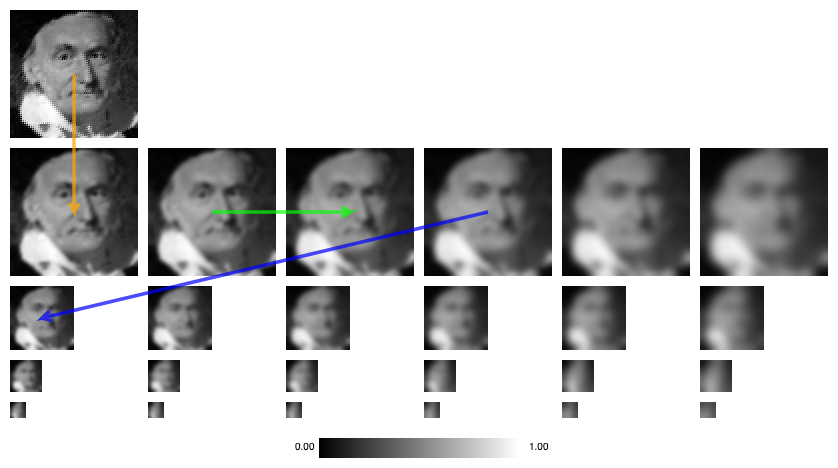
\includegraphics[width=\textwidth]{img/tracking/gauss-pyramide.png}
    \caption[Die Gauß-Pyramide für ein Eingangsbild. Das Bild wird runterskaliert und mit steigender Stärke mit einem Gauss-Weichzeichner versehen.]{Die Gauß-Pyramide für ein Eingangsbild. Das Bild wird runterskaliert und mit steigender Stärke mit einem Gauss-Weichzeichner versehen\protect\footnotemark.}
    \label{fig: tracking-gauss-pyramide}
\end{figure}

\footnotetext{Quelle Bild: http://weitz.de/sift/, zuletzt aufgerufen am 01.08.2022}

Dann werden nach \textit{Schlüsselpunkten (engl. Key Points, Feature Points)} in einem Bild gesucht. Es wird von je zwei benachbarten Bildern in der Gauß-Pyramide die Differenz gebildet (\textit{Difference of Gaussians (DoG)}). Dadurch entstehen Grauwerte, die diskrete Maximas erkennen lassen. Für jeden Punkt wird der Grauwert des mittleren Pixels mit den Grauwerten der umliegenden Pixel und die Grauwerte der benachbarten Bilder an der gleichen Stelle verglichen. Ist ein starker Unterschied bemerkbar, gilt der Punkt als Kanditat für einen Schlüsselpunkt. In Abbildung \ref*{fig:tracking-sift-features} werden Schlüsselpunkte gefunden. Die roten Punkte enthalten starke Extrema, die im weiteren Verlauf betrachtet werden. Die gelben Punkte enthalten zwar Extrema, jedoch sind die Unterschiede der Grauwerte so gering, dass sie unter dem eingestellten Schwellwert liegen und aussortiert werden. Diese werden beispielsweise als Rauschen erkannt. Je nachdem wie groß das Bild ist und wie stark die Schwellwerte beim jeweiligen Detektor eingestellt sind, verändert sich die Anzahl an Schlüsselpunkten. Dies beeinflusst die Tracking Performance und die Genauigkeit.
Wie?

\begin{figure}[H]
    \centering
    \subfloat[][]{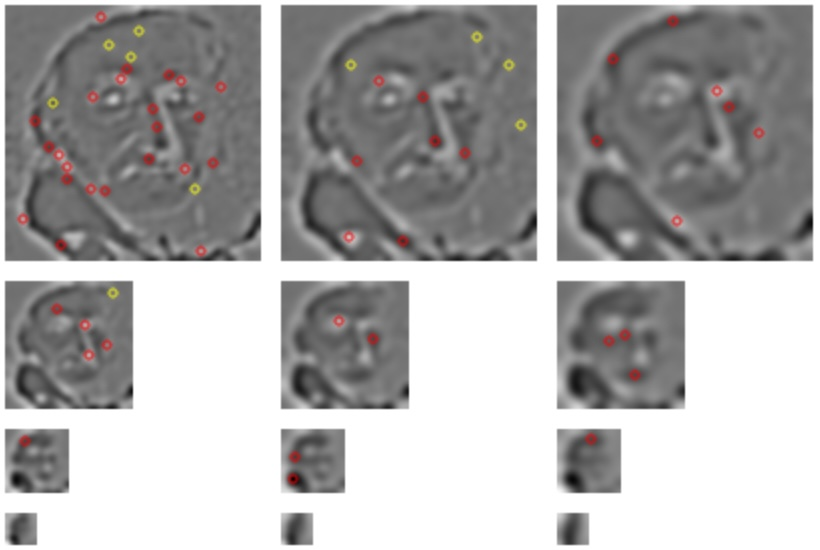
\includegraphics[width=0.4\linewidth]{img/tracking/feature-detection-sift.jpg}}%
    \qquad
    \subfloat[][]{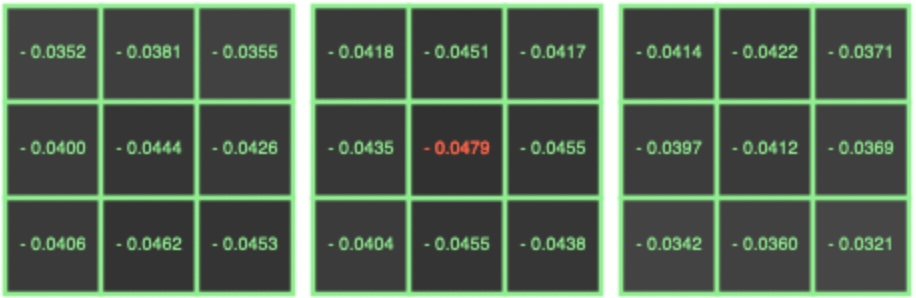
\includegraphics[width=0.4\linewidth]{img/tracking/feature-detection-sift-werte.jpg}}%
    \caption[Detektierte Schlüsselpunkte anhand der Extremas der DoG Bilder und deren Nachbarbilder (a) und die Grauwerte des Punktes auf der Nasenspitze der Person (b). Der Grauwert an der Stelle der Nase unterscheidet sich stark von seinen benachbarten Pixeln und beherbergt daher ein Extrema]{Detektierte Schlüsselpunkte anhand der Extremas der DoG Bilder und deren Nachbarbilder (a) und die Grauwerte des Punktes auf der Nasenspitze der Person (b). Der Grauwert an der Stelle der Nase unterscheidet sich stark von seinen benachbarten Pixeln und beherbergt daher ein Extrema\protect\footnotemark.}%
    \label{fig:tracking-sift-features}
\end{figure}

\footnotetext{Quelle Bild: http://weitz.de/sift/, zuletzt aufgerufen am 01.08.2022}

Nach der ersten Auswahl der Schlüsselpunkte wird die Positionen der Schlüsselpunkte verbessert. Dazu werden mit der Taylor-Formel Taylorpolynome gebildet. Diese werden in der Mathematik genutzt, Punkte in der Umgebung einer Funktion anzunähern\footnote{https://de.wikipedia.org/wiki/Taylor-Formel, zuletzt aufgerufen am 01.08.2022}. Mit den Polynomen werden die diskreten x- und y-Koordinaten durch Nachkommastellen verfeinert. Mit feineren Koordinaten wird der Punkt genauer erfasst und die Auswahl der Schlüsselpunkte wird ebenfalls verfeinert.

Ist eine finale Auswahl der Schlüsselpunkte erfolgt, erhält jeder Punkt einen sogenannten \textit{Deskriptor}. Dieser enthält lokale Eigenschaften auf dem Bild in der Umgebung des Punktes. Ziel eines Deskriptors ist es Schlüsselpunkte eindeutig zu beschreiben. Der Algorithmus nimmt jeden Schlüsselpunkt, berechnet in einem bestimmten viereckigen Bereich um den Punkt Gradienten. Ein Gradient bestimmt die Richtung und Steigung der größten Änderung\footnote{https://de.wikipedia.org/wiki/Gradient, zuletzt aufgerufen am 01.08.2022}. Die Gradienten werden in einem Histogramm gespeichert. Aus dem Histogramm wird ersichtlich, in welche Richtung die meisten Gradienten zeigen und es wird daraus eine Referenzrichtung dieses Punktes abgeleitet. Der gleiche Prozess wird im nächsten Schritt nochmals durchgeführt. Jetzt ist die Auswahl kreisförmig und das genutzte Koordinatensystem orientiert sich an der zuvor abgeleiteten Referenzrichtung. Es wird wieder eine Hauptrichtung der Gradienten bestimmt und die Gradienten werden in weitere Histogramme abgespeichert. Die Informationen sind dazu da, die Schlüsselpunkte rotationsinvariant zu machen \cite*[Herling und Broll(2011),][]{herling2011} \cite*[Weitz(2022),][]{weitz2022}. 

Der Deskriptor hat am Ende des Algorithmus folgende Informationen für jeden Schlüsselpunkt:

\begin{itemize}
    \item Die verfeinerten x- und y-Koordinaten,
    \item der Skalierungsfaktor,
    \item der Grad an Unschärfe,
    \item die Hauptrichtungen der Gradienten,
    \item normalisierte 4x4x8=128 8-bit integer Werte, die die Histogramme aus dem letzten Schritt darestellen.
\end{itemize}

Diese Informationen beschreiben jeden Schlüsselpunkt eindeutig. Der Punkt ist durch die Skalierungen skaleninvariant, wenig anfällig für Rauschen oder feine Strukturen und rotierungsinvariant.

\begin{figure}[H]
    \centering
    \subfloat[][]{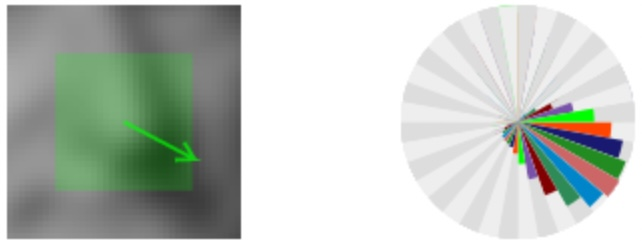
\includegraphics[width=0.4\linewidth]{img/tracking/feature-detection-sift-hauptrichtung.jpg}}%
    \qquad
    \subfloat[][]{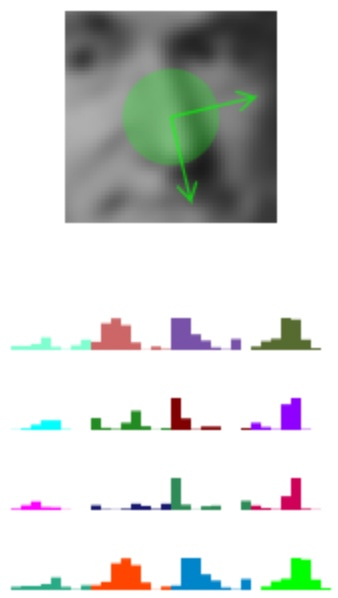
\includegraphics[width=0.4\linewidth]{img/tracking/feature-detection-histogramme.jpg}}%
    \caption[Das Histogramm und die Referenzrichtung im ersten Durchlauf (a) und das Koordinatensystem nach der Referenzrichtung und die entstandenen Histogramme(b).]{Das Histogramm und die Referenzrichtung im ersten Durchlauf (a) und das Koordinatensystem nach der Referenzrichtung und die entstandenen Histogramme(b)\protect\footnotemark.}%
    \label{fig:tracking-sift-richtungen}
\end{figure}

\footnotetext{Quelle Bild: http://weitz.de/sift/, zuletzt aufgerufen am 01.08.2022}

\subsubsubsection{Feature-Matching}

Sind die Deskriptoren vorhanden, kann im Anschluss ein \textit{Feature-Matching} durchgeführt werden. Dabei werden Schlüsselpunkte mit ihren Deskriptoren verglichen und zugeordnet. Mithilfe der zugeorndeten Schlüsselpunkten kann die Pose der Kamera berechnet werden \cite[Dörner(2019)][]{doerner}\cite[Herling und Broll(2011)][]{herling2011}. 

Als Beispiel wird mit Python\footnote{https://www.python.org/} und OpenCV\footnote{https://opencv.org/} ein Feature-Matching durchgeführt. Hierfür wird \acrshort{orb} verwendet. Abbildung \ref*{fig:orb-beispiel} zeigt das Feature-Matching Ergebnis mit der Brute Force Methode. Bei der Brute Force Methode werden die Deskriptoren verglichen. Der Deskriptor der, der am nächsten zum vergleichenden Deskriptor ist, wird zurückgegeben und als Match identifiziert\footnote{\url{https://docs.opencv.org/3.4/dc/dc3/tutorial_py_matcher.html}, zuletzt aufgerufen am 02.08.2022}. In diesem Beispiel wird die Skaleninvarianz und die Rotierungsinvarianz ersichtlich.

\begin{figure}[H]
    \centering
    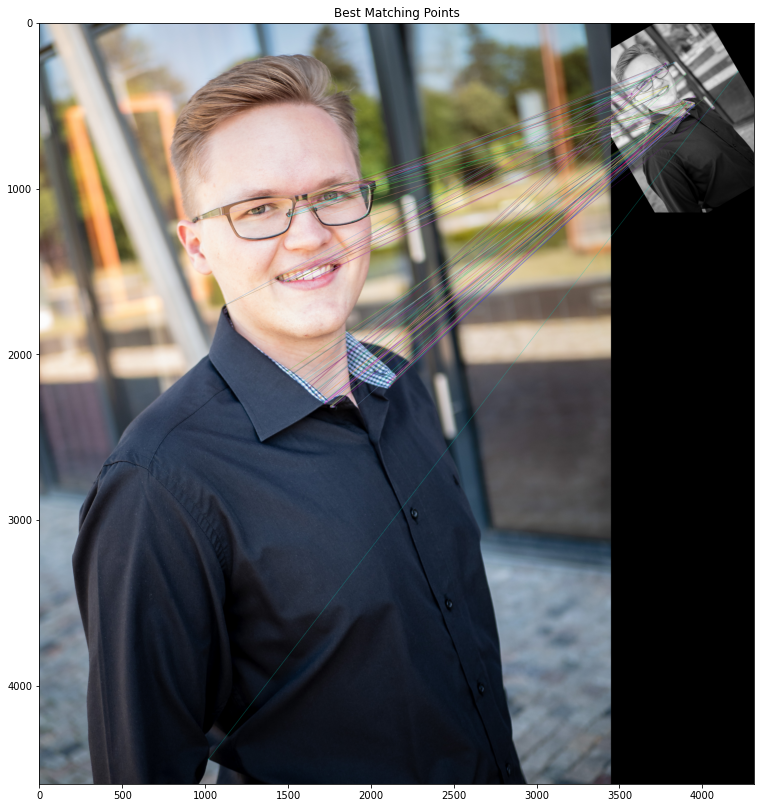
\includegraphics[width=10cm]{img/tracking/orb-3.png}
    \caption[Das Ergebnis des Feature-Matching mit ORB und OpenCV.]{Das Ergebnis des Feature-Matching mit ORB und OpenCV.\protect\footnotemark}
    \label{fig:orb-beispiel}
\end{figure}

\footnotetext{Link zum Source-Code:\\ \url{https://medium.com/data-breach/introduction-to-orb-oriented-fast-and-rotated-brief-4220e8ec40cf}, und das Beispiel: \url{https://github.com/Koliyoshii/masterarbeit/blob/main/opencv_orb_feature_matching.ipynb}}

\subsubsubsection{Simultaneous Localization and Mapping (SLAM)}
Während bei Feature-Matching Methoden eine Feature-Map für das Tracking vorhanden sein muss, verfolgt \acrshort{slam}\cite{slam1}\cite{slam2} einen weiterführenden Ansatz. So wird simultan zum Tracking eine Feature Map erstellt und kontinuierlich erweitert und verbessert. Während dem Tracking werden dreidimensionale Schlüsselpunkte ermittelt. Dabei wird entweder kamerabasiert (Visual SLAM) nach Merkmalen gesucht oder es kommen Sensoren zur Generierung von Tiefeninformationen, wie zum Beispiel \textit{LIDAR-Sensoren (engl. light detection and ranging)}, zum Einsatz\cite[Liu et al.][]{Liu2020}. Vorteil dieser Technik ist, dass bereits ab dem ersten Start eine grobe Positions- und Orientierungsbestimmung durchgeführt werden kann. Zusätzlich verbessert sich diese im Laufe des Trackings, indem immer weiter eine Karte mit 3D Schlüsselpunkten der Umgebung erstellt wird. Ursprünglich stammt SLAM aus der Robotertechnik, damit diese sich frei in einer Umgebung bewegen können. Da im AR-Kontext Smartphones weniger und unpräzisere Sensoren haben (z.B. keine Tiefensensoren) wird auf Visual SLAM gesetzt\cite[Dörner(2019) Seite 143 f., ][]{doerner}\cite[Herling und Broll(2011)][]{herling2011}. 

Weiterhin schlagen Klein und Murray\cite*{klein2007} das \textit{\acrfull{ptam}} für AR Anwendungen vor. Dabei wird die Idee von \acrshort{slam} mit einer einzelnen Kamera durchgeführt. Hierfür wird das Tracking über \acrshort{fast} und die Kartenerstellung aufgeteilt. Für jeden neuen Frame wird die Karte erweitert und 3D Schlüsselpunkte verbessert. Zusätzlich wird eine Hauptebene festgelegt, auf der die AR Objekte platziert werden. Diese Herangehensweise ist performant genug, um auf mobilen Geräten anwendung zu finden\cite[Klein und Murray(2009)][]{klein2009}. Auch ARCore richtet sich nach diesem Prinzip, indem Ebenen wie Tische oder Wände erkannt werden.

\subsubsection{Tracking in AR Core}
